\documentclass[11pt,letterpaper]{article}
\usepackage[utf8]{inputenc}
\usepackage[left=1in,right=1in,top=1in,bottom=1in]{geometry}
\usepackage{amsfonts,amsmath}
\usepackage{graphicx,float}
% -----------------------------------
\usepackage{hyperref}
\hypersetup{%
  colorlinks=true,
  linkcolor=blue,
  citecolor=blue,
  urlcolor=blue,
  linkbordercolor={0 0 1}
}
% -----------------------------------
\usepackage{fancyhdr}
\newcommand\course{MATH-UA.0252\\Numerical Analysis}
\newcommand\hwnumber{10}                  % <-- homework number
\newcommand\NetIDa{Ryan Sh\`iji\'e D\`u} 
\newcommand\NetIDb{November 18th, 2022}
\pagestyle{fancyplain}
\headheight 35pt
\lhead{\NetIDa\\\NetIDb}
\chead{\textbf{\Large Worksheet \hwnumber}}
\rhead{\course}
\lfoot{}
\cfoot{}
\rfoot{\small\thepage}
\headsep 1.5em
% -----------------------------------
\usepackage{titlesec}
\renewcommand\thesubsection{(\arabic{section}.\alph{subsection})}
\titleformat{\subsection}[runin]
        {\normalfont\bfseries}
        {\thesubsection}% the label and number
        {0.5em}% space between label/number and subsection title
        {}% formatting commands applied just to subsection title
        []% punctuation or other commands following subsection title
% -----------------------------------
\setlength{\parindent}{0.0in}
\setlength{\parskip}{0.1in}
% -----------------------------------
\newcommand{\de}{\mathrm{d}}
\newcommand{\DD}{\mathrm{D}}
\newcommand{\pe}{\partial}
\newcommand{\mcal}{\mathcal}
%\newcommand{\pdx}{\left|\frac{\partial}{\partial_x}\right|}

\newcommand{\dsp}{\displaystyle}

\newcommand{\norm}[1]{\left\Vert #1 \right\Vert}
%\newcommand{\mean}[1]{\left\langle #1 \right\rangle}
\newcommand{\mean}[1]{\overline{#1}}
\newcommand{\inner}[2]{\left\langle #1,#2\right\rangle}

\newcommand{\ve}[1]{\boldsymbol{#1}}

\newcommand{\thus}{\Rightarrow \quad }
\newcommand{\fff}{\iff\quad}
\newcommand{\qdt}[1]{\quad \mbox{#1} \quad}

\renewcommand{\Re}{\mathrm{Re}}
\renewcommand{\Im}{\mathrm{Im}}
\newcommand{\E}{\mathbb{E}}
\newcommand{\lap} {\nabla^2}
\renewcommand{\div}{\nabla\cdot}

\newcommand{\csch}{\text{csch}}
\newcommand{\sech}{\text{sech}}


\newcommand{\hot}{\text{h.o.t.}}

\newcommand{\ssp}{\left.\qquad\right.}

\newcommand{\var}{\text{var}}
\newcommand{\cov}{\text{cov}}

%%%%%%%%%%%%%%%%%%%%%%%%%%%%%%%%%%%%%%%%%%%%%%%%%%
\makeatletter
\newcommand*{\mint}[1]{%
  % #1: overlay symbol
  \mint@l{#1}{}%
}
\newcommand*{\mint@l}[2]{%
  % #1: overlay symbol
  % #2: limits
  \@ifnextchar\limits{%
    \mint@l{#1}%
  }{%
    \@ifnextchar\nolimits{%
      \mint@l{#1}%
    }{%
      \@ifnextchar\displaylimits{%
        \mint@l{#1}%
      }{%
        \mint@s{#2}{#1}%
      }%
    }%
  }%
}
\newcommand*{\mint@s}[2]{%
  % #1: limits
  % #2: overlay symbol
  \@ifnextchar_{%
    \mint@sub{#1}{#2}%
  }{%
    \@ifnextchar^{%
      \mint@sup{#1}{#2}%
    }{%
      \mint@{#1}{#2}{}{}%
    }%
  }%
}
\def\mint@sub#1#2_#3{%
  \@ifnextchar^{%
    \mint@sub@sup{#1}{#2}{#3}%
  }{%
    \mint@{#1}{#2}{#3}{}%
  }%
}
\def\mint@sup#1#2^#3{%
  \@ifnextchar_{%
    \mint@sup@sub{#1}{#2}{#3}%
  }{%
    \mint@{#1}{#2}{}{#3}%
  }%
}
\def\mint@sub@sup#1#2#3^#4{%
  \mint@{#1}{#2}{#3}{#4}%
}
\def\mint@sup@sub#1#2#3_#4{%
  \mint@{#1}{#2}{#4}{#3}%
}
\newcommand*{\mint@}[4]{%
  % #1: \limits, \nolimits, \displaylimits
  % #2: overlay symbol: -, =, ...
  % #3: subscript
  % #4: superscript
  \mathop{}%
  \mkern-\thinmuskip
  \mathchoice{%
    \mint@@{#1}{#2}{#3}{#4}%
        \displaystyle\textstyle\scriptstyle
  }{%
    \mint@@{#1}{#2}{#3}{#4}%
        \textstyle\scriptstyle\scriptstyle
  }{%
    \mint@@{#1}{#2}{#3}{#4}%
        \scriptstyle\scriptscriptstyle\scriptscriptstyle
  }{%
    \mint@@{#1}{#2}{#3}{#4}%
        \scriptscriptstyle\scriptscriptstyle\scriptscriptstyle
  }%
  \mkern-\thinmuskip
  \int#1%
  \ifx\\#3\\\else_{#3}\fi
  \ifx\\#4\\\else^{#4}\fi  
}
\newcommand*{\mint@@}[7]{%
  % #1: limits
  % #2: overlay symbol
  % #3: subscript
  % #4: superscript
  % #5: math style
  % #6: math style for overlay symbol
  % #7: math style for subscript/superscript
  \begingroup
    \sbox0{$#5\int\m@th$}%
    \sbox2{$#5\int_{}\m@th$}%
    \dimen2=\wd0 %
    % => \dimen2 = width of \int
    \let\mint@limits=#1\relax
    \ifx\mint@limits\relax
      \sbox4{$#5\int_{\kern1sp}^{\kern1sp}\m@th$}%
      \ifdim\wd4>\wd2 %
        \let\mint@limits=\nolimits
      \else
        \let\mint@limits=\limits
      \fi
    \fi
    \ifx\mint@limits\displaylimits
      \ifx#5\displaystyle
        \let\mint@limits=\limits
      \fi
    \fi
    \ifx\mint@limits\limits
      \sbox0{$#7#3\m@th$}%
      \sbox2{$#7#4\m@th$}%
      \ifdim\wd0>\dimen2 %
        \dimen2=\wd0 %
      \fi
      \ifdim\wd2>\dimen2 %
        \dimen2=\wd2 %
      \fi
    \fi
    \rlap{%
      $#5%
        \vcenter{%
          \hbox to\dimen2{%
            \hss
            $#6{#2}\m@th$%
            \hss
          }%
        }%
      $%
    }%
  \endgroup
}

\begin{document}

\section{Singular Value Decomposition (SVD) basics}
\subsection{}
Like QR, SVD has the full and reduced form \cite{TrefethenBau_97}:
\begin{figure}[H]
    \centering
    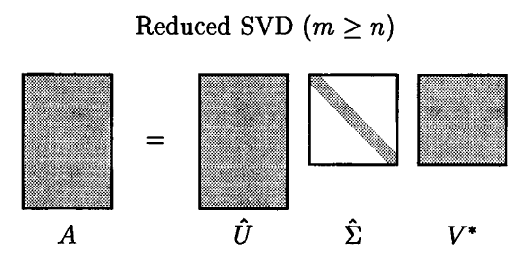
\includegraphics[width = 0.49\textwidth]{figs/TB_reducedSVD}
    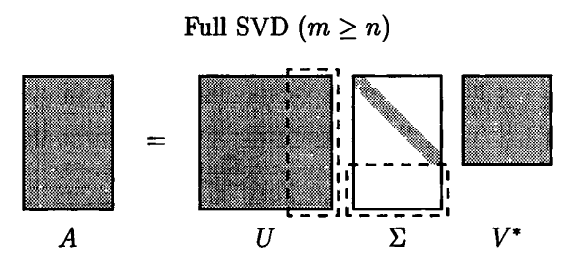
\includegraphics[width = 0.49\textwidth]{figs/TB_fullSVD}
\end{figure}
Note that the full form has $U$ which spans the whole of $\mathbb{R}^n$.

\subsection{}
We can interpret the full form of SVD as a change of basis, then a scaling, and then another change of basis (Figure from \cite{Strang_93}).
\begin{figure}[H]
    \centering
    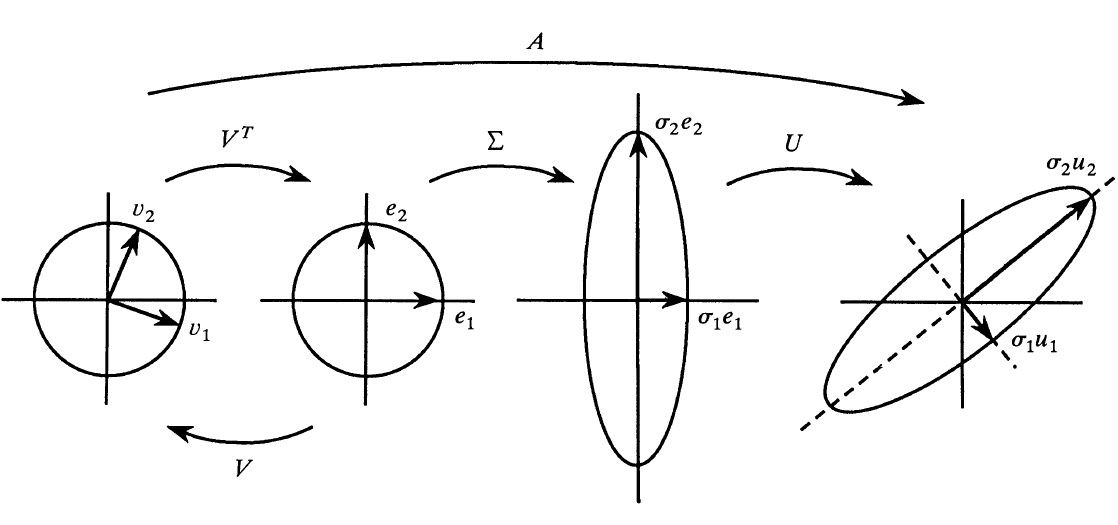
\includegraphics[width = 0.7\textwidth]{figs/strang_SVD}
\end{figure}

\section{Some properties of SVD}
We list (and attempt to prove) some properties of SVD:

\subsection{}
$\text{range}(A) = \text{span}(\ve u_1,\ve u_2,\dots,\ve u_r)$ and $\text{null}(A) = \text{span}(\ve v_{r+1},\dots,\ve v_n)$. 

\subsection{}
The rank of $A$ is $r$, the number of nonzero singular values.

\subsection{}
We have $\norm{A}_2 = \sigma_1$, the largest singular value. And $\norm{A}_F = \sqrt{\sigma_1^2+\sigma_2^2+\dots+\sigma_r^2}$. 

You will show the second property in your homework.

\section{Low-rank approximation using SVD}
\subsection{}
Show that $A$ is the sum of $r$ \emph{rank-one} matrices:
\begin{align*}
    A = \sum_{j=1}^r \sigma_j \ve u_j \ve v_j^\top.
\end{align*}

\subsection{}
For any $\nu$ with $0\leq \nu \leq r$, define
\begin{align*}
    A_\nu = \sum_{j=1}^\nu \sigma_j \ve u_j \ve v_j^\top.
\end{align*}
Then we have
\begin{align*}
    \norm{A-A_\nu}_2 = \inf_{\substack{B\in\mathbb{R}^{m\times n}\\\text{rank}(B)\leq\nu}}\norm{A-B}_2 = \sigma_{\nu+1}.
\end{align*}

Note that a similar theorem is also true for the Frobenius norm.

\section{Polynomial interpolation and linear algebra}
In lecture you have learned the theorem which states:

For $n\geq 1$ and distinct $n+1$ data pairs $(x_0,y_0),\dots,(x_n,y_n)$ there exists a unique $p_n(x)\in P_n$, an $n$-th order polynomial such that $p_n(x_i) = y_i$ for $i = 0,\dots,n$. 

We will try to prove this using linear algebra.

\subsection{}
We can write an $n$-th order polynomial as
\begin{align*}
    p_n(x) = a_0 + a_1x + \dots + a_nx^n.
\end{align*}
This gives us $n+1$ free variables to solve. Frame the problem of finding $p_n(x)$ s.t. $p_n(x_i) = y_i$ for $i = 0,\dots,n$ as a matrix problem $X\ve a = \ve y$.

\subsection{}
Show that since $x_i\neq x_j$ for all $i,j$, we have the matrix $X$ we constructed has full rank. 

\subsection{}
Think about the uniqueness and existence claim in the theorem in linear algebra language. 


\vfill
\bibliographystyle{alpha}
\bibliography{citation}

\end{document}